\section{Universality \& Completeness}

As statet in \cite{duncan2020simplification} the ZX-Calculus is universal, because any linear map can be represented as a ZX-diagram. This means that any valid quantum circuit can be represented as a ZX-diagram. Additionally it can be shown that ZX-Calculus is complete for circuits which are expressed using the \textit{Clifford+T} gates. This means that any two circuits in this family can be transformed into each other by a series of rewrite rules from above.
In particular this means, that if a simplified version of the circuit exists, it can be found by the rules of the ZX-Calculus. Such a simplification process is shown in figure \ref{fig:simplification-idea}.

\begin{figure}[h]
    \centering
    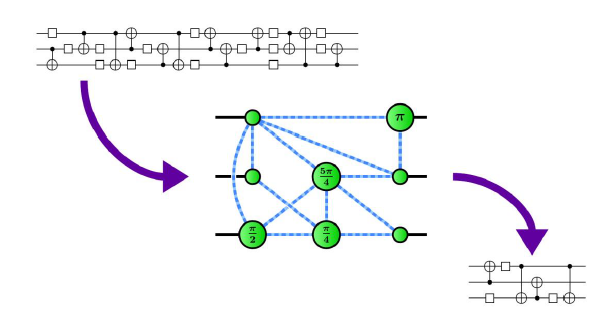
\includegraphics[width=0.45\textwidth]{images/simplification-idea.png}
    \caption{Simplification process\cite{duncan2020simplification-image}}
    \label{fig:simplification-idea}
\end{figure}